%----------------------------------------------------------------------------
\chapter{Data}
\label{chap:data}
%----------------------------------------------------------------------------

%----------------------------------------------------------------------------
\section{ogbn-arxiv and its limitations}
\label{sec:ogbn-arxiv}
%----------------------------------------------------------------------------

The starting point is ogbn-arxiv, a citation graph from the Open Graph Benchmark~\cite{hu2020open}. It contains 169,343 computer science papers from arXiv and 1,166,243 directed citation edges between them, and it was built from the Microsoft Academic Graph (MAG)~\cite{hu2020open,wang2020microsoft}. Each edge points from a paper to a paper it cites~\cite{hu2020open}. Each paper has a MAG identifier, a title, an abstract and a publication year. The dataset also assigns each paper a subject category, which this thesis does not use.

The recorded citations are sparse. Counting the recorded references, I found that a paper cites an average of 6.89 other papers in the graph, with a median of 4. For 17,440 papers, about 10\% of the dataset, no outgoing citation is recorded at all, and only 499 papers have more than 50.

These counts do not necessarily reflect the length of a paper's bibliography, because ogbn-arxiv records only citations between papers included in the dataset~\cite{hu2020open}. A reference to a journal or conference paper that is not on arXiv, to a book, or to a paper from another field is therefore missing. The task in this thesis is to generate a paper's abstract from the papers it cites (\autoref{chap:task}). Missing references therefore limit the information available to the model. To include references beyond the papers in ogbn-arxiv, I enriched the graph with citation records from another source.

%----------------------------------------------------------------------------
\section{Enrichment with Semantic Scholar}
\label{sec:enrichment}
%----------------------------------------------------------------------------

The additional citation records come from Semantic Scholar, an open data platform for scholarly literature that releases its data as bulk datasets~\cite{kinney2023semantic}. I used three of them: the paper records, the abstracts and the citations. Within Semantic Scholar, these records are connected by the Corpus ID, Semantic Scholar's identifier for a paper, so I linked each abstract to its paper record using the Corpus ID. The paper record also provides the MAG identifier, which connects the paper to ogbn-arxiv. For each citation, I used the paper records to obtain the MAG identifiers of both the citing and the cited paper. \autoref{fig:enrichment}a illustrates this matching: the ogbn-arxiv paper with MAG identifier 100 is matched to the Semantic Scholar record with Corpus ID 700, and a citation record from Corpus ID 700 to Corpus ID 900, whose paper record gives MAG identifier 200, becomes a citation from MAG identifier 100 to MAG identifier 200.

In what follows, I call the 169,343 papers of ogbn-arxiv \emph{ogbn-arxiv papers} and the papers contributed by Semantic Scholar \emph{added papers}. The graph was then expanded in four steps (\autoref{fig:enrichment}b). First, I collected the papers that the ogbn-arxiv papers cite according to Semantic Scholar. Second, I added referenced papers absent from ogbn-arxiv when Semantic Scholar provided both a MAG identifier and an abstract. Third, I kept every Semantic Scholar citation between two papers of the resulting set for which Semantic Scholar provided both. Fourth, I combined these citations with the original edges of ogbn-arxiv and removed duplicates. All papers and edges of ogbn-arxiv are preserved, including those for which Semantic Scholar provides no MAG identifier or abstract. I did not repeat this expansion for the added papers. Their references were retained only when the cited paper was already in the selected set.

\begin{figure}[!ht]
  \centering
  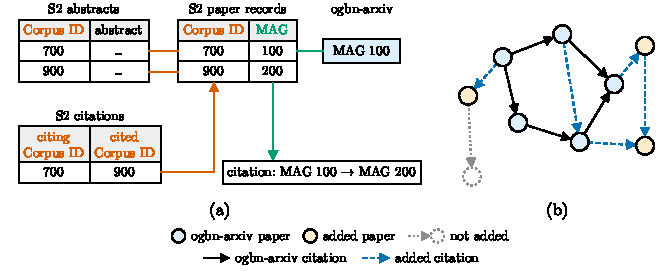
\includegraphics[width=\textwidth]{../diagrams/figures/data/enrichment.pdf}
  \caption{Building the joint graph. (a)~Abstracts and citation records are linked through Semantic Scholar's Corpus IDs, while MAG identifiers connect papers to ogbn-arxiv. Identifiers are illustrative; orange lines indicate Corpus ID matches and green lines indicate MAG matches. (b)~Eligible papers cited by ogbn-arxiv papers are added, together with Semantic Scholar citations between retained papers. Expansion is not recursive. Arrows point from citing to cited papers.}
  \label{fig:enrichment}
\end{figure}

The two groups of papers play different roles. Only ogbn-arxiv papers are prediction targets. Added papers enter the graph because an ogbn-arxiv paper cites them, and they serve only as additional neighbourhood information. When a paper appears in both sources, its title, abstract and year are taken from ogbn-arxiv. I checked that the two sources record citations in the same direction and that the joint graph contains no duplicate papers or edges. The joint graph has 384,756 papers, 169,343 from ogbn-arxiv and 215,413 added, and 3,844,151 directed citation edges in total.

\autoref{tab:enrichment} compares the recorded references of the ogbn-arxiv papers before and after the enrichment. The median number of recorded references per paper doubles, from 4 to 8, while the mean rises from 6.89 to 12.55, and the number of papers without any recorded reference is approximately halved. The citations made by ogbn-arxiv papers grow from 1,166,243 to 2,125,355: 889,024 of the new ones point to added papers, and 70,088 connect two ogbn-arxiv papers whose citation ogbn-arxiv had not recorded. The other 1,718,796 edges of the joint graph are citations made by added papers.

\begin{table}[!ht]
  \centering
  \begin{tabular}{lrr}
    \toprule
    Property of the ogbn-arxiv papers & Before & After \\
    \midrule
    Mean recorded references & 6.89 & 12.55 \\
    Median recorded references & 4 & 8 \\
    Papers with no recorded reference & 17,440 & 8,675 \\
    Papers with more than 50 recorded references & 499 & 4,284 \\
    \bottomrule
  \end{tabular}
  \caption{Recorded references of the 169,343 ogbn-arxiv papers in ogbn-arxiv alone (before) and in the joint graph (after the enrichment with Semantic Scholar).}
  \label{tab:enrichment}
\end{table}

The enrichment is uneven, however (\autoref{fig:enrichment-degree}). Semantic Scholar added at least one citation to 94,756 ogbn-arxiv papers (56\%), which have on average 17.0 recorded references in the joint graph. The other 74,587 papers (44\%) keep only the citations recorded in ogbn-arxiv, on average 6.9; 4,055 of them have a Semantic Scholar record with a MAG identifier and an abstract, but it added no new citation. A low number of recorded references therefore does not necessarily mean a short bibliography: it can also mean that the bibliography was only partly observed. The recorded reference count alone cannot distinguish these explanations. I retained papers that gained no additional citations, because excluding them would restrict the study to papers whose recorded neighbourhoods were expanded by Semantic Scholar. The implications of this uneven coverage are discussed with the limitations of the results \textcolor{red}{[TODO: reference to the discussion chapter]}.

\begin{figure}[!ht]
  \centering
  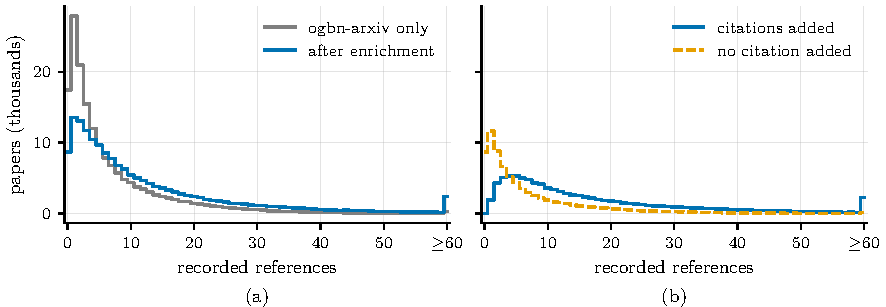
\includegraphics{../diagrams/figures/data/enrichment_degree.pdf}
  \caption{Number of recorded references per ogbn-arxiv paper. (a)~In ogbn-arxiv alone and after the enrichment with Semantic Scholar. (b)~After the enrichment, separately for the papers to which Semantic Scholar added at least one citation and for the others, which keep only the citations recorded in ogbn-arxiv. The last bin contains papers with 60 or more recorded references.}
  \label{fig:enrichment-degree}
\end{figure}


%----------------------------------------------------------------------------
\section{The graph used by the model}
\label{sec:model-graph}
%----------------------------------------------------------------------------

In the joint graph, a citation edge points from the paper making the citation to the paper being cited. For example, if paper A cites paper B, the recorded edge is A $\rightarrow$ B. To generate A's abstract, however, the model needs information from B. I therefore reverse the edges for message passing, so that information flows from cited papers into the papers that cite them (\autoref{fig:message-passing}).

This direction also restricts the model to a target paper's references. Papers that later cite the target may contain information about its findings that was unavailable when its abstract was written. Allowing information to flow in both directions would make those later papers available to the model and introduce temporal leakage.

All experiments use the same joint graph. The training, validation and evaluation sets divide the prediction targets rather than the graph itself. A paper assigned to one set can therefore supply reference information to a target in another set. In particular, a validation or evaluation paper can appear among a training paper's references. Its embedding then supplies neighbourhood information, although its abstract is not used as a training target.

I removed citation self-loops, which connect a paper to itself, so that a target cannot appear among its own references. This removal does not replace the masking of the target's own embedding, which is described in \autoref{sec:gnn-estimator}. The model uses every recorded reference of a target, without sampling or imposing a neighbourhood-size cap.

%----------------------------------------------------------------------------
\section{Exploring the joint graph}
\label{sec:exploration}
%----------------------------------------------------------------------------

After enrichment, an ogbn-arxiv paper has a median of eight recorded references (\autoref{fig:enrichment-degree}). Most papers have relatively few references, but a small number have much larger bibliographies: 391 papers have more than 100 recorded references, with a maximum of 832. The amount of reference information available to the model therefore varies considerably between targets.

Many papers share references to widely cited works. Among the ogbn-arxiv papers, 19\% cite at least one of the ten most cited papers in the joint graph. These widely cited works therefore appear as input to many different targets.

The model generates abstracts for selected ogbn-arxiv papers, while the abstracts of cited papers provide input information. Across all ogbn-arxiv papers, the median abstract length is 157 words, and the middle 80\% contain between 91 and 237 words. Added papers also have a median abstract length of 157 words, indicating that the enrichment introduces abstracts of similar typical length.

\autoref{tab:example} illustrates the task using ``On the Power of Curriculum Learning in Training Deep Networks'' by Hacohen and Weinshall~\cite{hacohen2019power}. I selected this example for clarity rather than representativeness. The table shows the shortened abstract and the titles of its eleven recorded references. The model's reference representations use both titles and abstracts; only titles are displayed here for readability.

\begin{table}[!ht]
  \centering
  \small
  \begin{tabular}{rp{0.8\textwidth}}
    \toprule
    \multicolumn{2}{p{0.88\textwidth}}{\textit{Abstract (shortened):} ``[\ldots] In this work, we analyze the effect of curriculum learning, which involves the non-uniform sampling of mini-batches, on the training of deep networks, and specifically CNNs trained for image recognition. To employ curriculum learning, the training algorithm must resolve 2 problems: (i) sort the training examples by difficulty; (ii) compute a series of mini-batches that exhibit an increasing level of difficulty. We address challenge (i) using two methods: transfer learning from some competitive `teacher' network, and bootstrapping. [\ldots] We address challenge (ii) by investigating different pacing functions to guide the sampling. [\ldots] We conclude with a novel theoretical analysis of curriculum learning, where we show how it effectively modifies the optimization landscape. [\ldots]''} \\
    \midrule
    Year & Recorded reference \\
    \midrule
    2014 & learning to execute \\
    2014 & very deep convolutional networks for large scale image recognition \\
    2015 & cyclical learning rates for training neural networks \\
    2015 & rethinking the inception architecture for computer vision \\
    2015 & deep speech 2 end to end speech recognition in english and mandarin \\
    2015 & deep residual learning for image recognition \\
    2017 & automated curriculum learning for neural networks \\
    2017 & reverse curriculum generation for reinforcement learning \\
    2017 & mentornet learning data driven curriculum for very deep neural networks on corrupted labels \\
    2018 & curriculum learning by transfer learning theory and experiments with deep networks \\
    2018 & learning to teach \\
    \bottomrule
  \end{tabular}
  \caption{An example from the evaluation set, chosen for clarity: the shortened abstract of Hacohen and Weinshall~\cite{hacohen2019power} and the titles of its eleven recorded references, all of them ogbn-arxiv papers. The titles are given as ogbn-arxiv records them, in lower case and without punctuation.}
  \label{tab:example}
\end{table}

Four of the eleven reference titles explicitly mention curriculum learning, while others concern deep neural networks and image recognition. The references therefore make the broad topic recognisable. The target abstract goes further by describing the paper's own methods and findings, including ways to order training examples by difficulty and an analysis of pacing functions. These details are not apparent from the reference titles alone.

\newpage
%----------------------------------------------------------------------------
\section{Node text and embeddings}
\label{sec:embeddings}
%----------------------------------------------------------------------------

To use the papers' text as node features in the graph, I converted each paper's title and abstract into a single vector. An embedding model is a neural network that maps a piece of text to a vector of fixed length. It is trained so that texts with similar meaning are mapped to vectors that point in similar directions. The similarity of two such vectors $\mathbf{u}$ and $\mathbf{v}$ is measured by their cosine similarity, the cosine of the angle between them:
\[
  \cos(\mathbf{u}, \mathbf{v}) = \frac{\mathbf{u}^\top \mathbf{v}}{\lVert \mathbf{u} \rVert \, \lVert \mathbf{v} \rVert}.
\]
It is 1 for vectors that point in the same direction, 0 for orthogonal vectors and $-1$ for vectors that point in opposite directions. For vectors of unit length, it equals their dot product.

I embedded every paper of the joint graph, ogbn-arxiv papers and added papers alike, with the \texttt{voyage-4-large} model~\cite{voyage2026voyage4}. The input text is the title of the paper followed by its abstract, separated by a blank line. I used the document input type, with which the model prepends a fixed instruction for representing documents to the text~\cite{voyage2026embeddings}. Each paper is thus represented by a 1024-dimensional vector of unit length. Representing the title and abstract together gives each node a compact representation of the paper's content. The embeddings are computed from the original text, before the cleaning of the training targets described in \autoref{sec:cleaning}.

These embeddings are the node features of the graph. When a paper appears among the references of a target, its embedding is the information it contributes to that target.

Randomly selected papers also have positive cosine similarities in this embedding space. Across 100,000 random pairs from the joint graph, the median similarity is 0.29, and 90\% of the pairs lie between 0.17 and 0.44. Shared scientific vocabulary, writing style and overlapping topics may contribute to this similarity, although this analysis does not establish their individual effects. A positive cosine similarity alone therefore does not show that two papers are closely related: it must be interpreted relative to the similarity of randomly selected papers. The later analysis examines whether a paper is more similar to the combined representation of its own references than to those of other papers.

%----------------------------------------------------------------------------
\section{Splits and node sets}
\label{sec:splits}
%----------------------------------------------------------------------------

I retained the predefined training, validation and test partitions of ogbn-arxiv, which are based on publication year~\cite{hu2020open}. The experimental node sets were selected within these partitions, without moving papers between them. Only ogbn-arxiv papers are prediction targets.

To examine generation across different neighbourhood sizes, I selected up to ten test papers for each recorded reference count from 5 to 100, using a fixed random seed. Where fewer than ten papers were available, I included them all. This produced 945 evaluation papers. Applying the same procedure within the validation partition produced 806 validation papers, which are used to monitor training. This sampling gives greater representation to papers with many references than they have in the full dataset. Aggregate evaluation scores therefore describe this selected population rather than the original distribution of ogbn-arxiv papers.

The training set contains every paper of the training partition, with two exceptions. I removed 477 papers whose abstracts have fewer than 30 words, to exclude very short or incomplete abstracts. I also removed three near-duplicates of evaluation papers, identified by the same normalised title or an embedding cosine similarity above 0.95, because training on them could expose the model to an evaluation target. This leaves 90,461 training papers. The three sets do not overlap, and all of them are stored in fixed files, so every experiment uses the same papers. The GNN is trained only on the 83,259 training papers with at least one recorded reference, because the other papers provide no reference information for the GNN to aggregate.

The training set retains almost all papers in the original training partition and is dominated by papers with few recorded references: the median is 5 and the mean is 7.9. In contrast, the evaluation sampling spreads papers across reference counts from 5 to 100, producing a mean of 51.8. The evaluation therefore places more emphasis on larger neighbourhoods than the training distribution does.

\subsection{Semantic information in the references}
\label{sec:reference-information}

For each evaluation paper, I averaged the embeddings of its recorded references and call the resulting vector its reference mean. I then compared the paper's similarity to this vector with its similarity to the reference means of the other evaluation papers (\autoref{fig:reference-mean-cosine}). The paper's own reference mean reaches a mean cosine similarity of 0.823, whereas the reference means of the other 944 evaluation papers reach 0.496. For 98.9\% of evaluation papers, similarity to their own reference mean exceeds the 95th percentile of the pooled baseline distribution. On the validation set, the corresponding means are 0.816 and 0.488.

\begin{figure}[!ht]
  \centering
  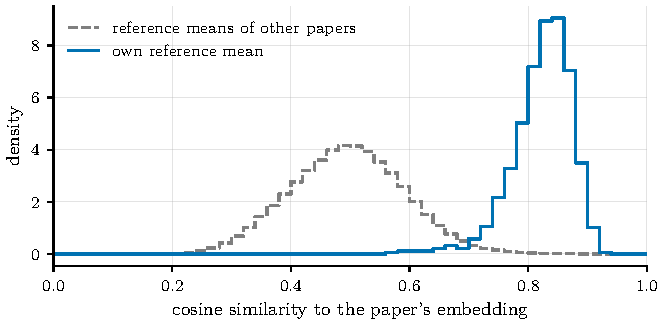
\includegraphics{../diagrams/figures/data/reference_mean_cosine.pdf}
  \caption{Cosine similarity between the embedding of each of the 945 evaluation papers and the mean embedding of its own recorded references, compared with its similarity to the reference means of the other 944 evaluation papers. Both distributions are normalised to unit area.}
  \label{fig:reference-mean-cosine}
\end{figure}

The references therefore carry information specific to the paper, beyond the similarity shared by papers in general. This is evidence of semantic similarity, which motivates recovering the content of a paper from its references. It does not show that the references contain every detail of the paper's abstract.

%----------------------------------------------------------------------------
\section{Cleaning the training targets}
\label{sec:cleaning}
%----------------------------------------------------------------------------

The abstracts on arXiv are written by the authors themselves and often contain LaTeX markup: mathematical expressions between dollar signs, commands that format text, and accents written as escape sequences. The instruction that the language model receives asks for plain prose without markup or mathematical notation. If the abstracts used as training targets kept their markup, the instruction and the examples from which the model learns would contradict each other. I therefore cleaned the abstracts that serve as training targets.

The cleaning removes LaTeX formatting while retaining the enclosed text and mathematical expressions where possible. It proceeds in five steps. First, it unwraps text-formatting commands such as \texttt{\textbackslash emph\{\ldots\}}, keeping the formatted text. Second, it removes the delimiters of mathematical expressions, but not the expressions themselves. Third, it replaces escaped characters such as \texttt{\textbackslash\%} with the characters themselves and drops accent marks. Fourth, it removes the backslash of any remaining command while keeping the command's name. Finally, it removes leftover braces and repeated whitespace. Keeping the content matters, because mathematical expressions and command names often describe the method or the result of a paper, which the target abstract should still contain. For example, \texttt{\$\textbackslash Omega(N \textbackslash log\textbackslash log N)\$} becomes ``Omega (N log log N)'' instead of disappearing.

Cleaning is applied to the training targets to match the requested output format. The node embeddings described in \autoref{sec:embeddings} are computed from the original titles and abstracts, preserving the source notation rather than incorporating the changes introduced by the cleaning rules. The input representation and the training target therefore come from different versions of the same abstract: the original text provides the node features, while the cleaned text provides an example of the desired output. Evaluation abstracts remain unchanged, so all experiments are scored against the same reference texts.
